\documentclass[11pt, oneside]{book}

% URLs and hyperlinks ---------------------------------------
\usepackage{hyperref}
\hypersetup{
	colorlinks=true,
	linkcolor=blue,
	filecolor=magenta,      
	urlcolor=blue,
}
\usepackage{xurl}
%---------------------------------------------------

% titlepage -------------------------------------------------
\usepackage{pdfpages}
%------------------------------------------------------------

% tables -------------------------------------------------------
\usepackage{float}
\usepackage{multirow}
\renewcommand{\arraystretch}{1.23}
% ---------------------------------------------------------------------

% commands --------------------------------------------
\newcommand{\amz}{\lr{Amazon} }
% -----------------------------------------------------------

\usepackage{xepersian}
\settextfont{Yas}
\setdigitfont{Yas}

\begin{document}
\frontmatter

\includepdf{../titlepage/title}
\tableofcontents
\mainmatter

\chapter{معرفی}
    پس از بررسی مواردی که برای پیاده‌سازی ارائه شده بود، موضوع \textit{منابع انسانی:‌ سیستم ارزیابی عملکرد کارمندان} انتخاب گردید.
    
    به طور خلاصه این سیستم قرار است طبق چارت سازمانی معرفی شده در ادامه‌ی این سند، خدمات آماری به همراه جزئیات، به شرکت \amz و مدیران آن ارائه دهد. 
    
    داده‌های مورد نیاز این خدمات آماری از آمار‌های ارائه شده توسط خود شرکت \amz و تمامی بازخورد (\lr{feedback})های مشتریان آن، جمع‌آوری و استفاده می‌شوند.
    
    بر این اساس چون این سیستم قرار است به بررسی عملکرد کارمندان شرکت \amz بپردازد، و خدماتی که ارائه می‌دهد، خدمات آماری هستند، نام \lr{\textit{Amazon Analytics}} برای آن انتخاب گردید.
    
    معرفی جامع و تکمیلی در سند \lr{Business Case}، در فصل \nameref{business-case} آورده شده است.
    
\chapter{مدل تجاری \lr{(Business Case)}}\label{business-case}
سند \lr{Business Case} به صورت یک فایل \lr{PDF} جداگانه نوشته شده، اما در همین فصل هم به طور کامل آورده شده تا براحتی به آن دسترسی داشته باشید. برای دسترسی به فایل جداگانه‌ی \lr{Business Case} به آدرس:
\begin{flushleft}
    \url{https://github.com/mahdihaghverdi/amazon-analytics/blob/main/business-case/business-case.pdf}
\end{flushleft}
مراجعه کنید.


\includepdf[page=-]{../business-case/business-case}

\chapter{پیاده‌سازی نسخه‌ی دمو}
از آنجایی که سیستم 
\lr{Amazon Analytics}
یک سیستم تمام آنالیزی‌ست و کارش ارائه‌ی آمار و تحلیل‌هاست، تیم ما دنبال یک پلتفرم بود که بتواند دیتا دریافت کند و خروجی‌هایی مانند نمودارها و چارت‌ها ارائه دهد که پس از تحقیق بسیار به پلتفرم
\url{amplitude.com}
رسیدیم که پلتفرم خوبی برای ارائه‌ی نسخه‌ی دمو هست.

\chapter{قالب \lr{Brainstorming}}
قالب بارش فکری که در \lr{Confluence} نوشته شده در این فصل آورده شده است. برای دسترسی به فایل جداگانه به آدرس:
\begin{flushleft}
    \url{https://github.com/mahdihaghverdi/amazon-analytics/blob/main/confluence/AA-Brainstorming-231023-135340.pdf}
\end{flushleft}
مراجعه کنید.

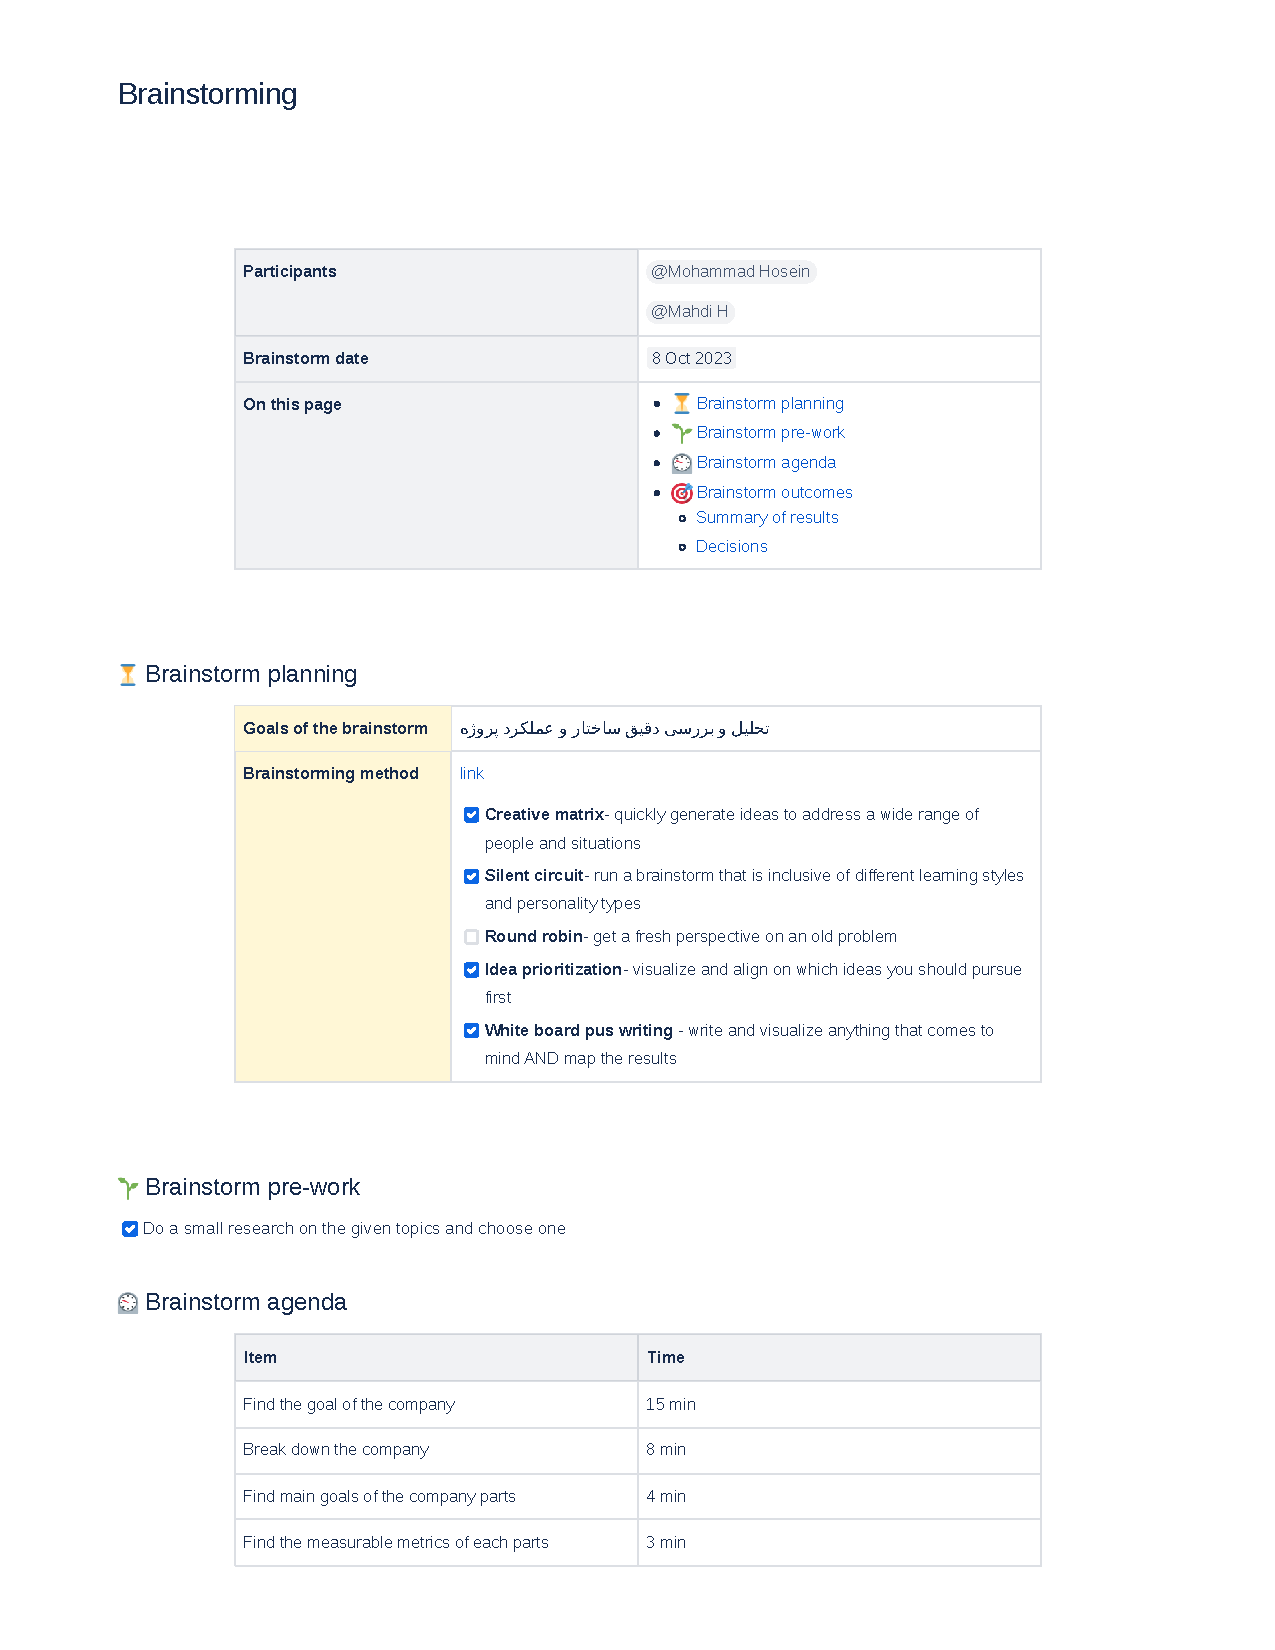
\includepdf[page=-]{../confluence/AA-Brainstorming-231023-135340}
\end{document}